\documentclass[tikz,border=8pt]{standalone}
% Shared look for every TikZ diagram. Load with \input{../../tools/tikz-style.tex}
\usepackage[sfdefault]{roboto}
\usetikzlibrary{arrows.meta, positioning, shapes.geometric, calc, fit, backgrounds}
\definecolor{cblue}{HTML}{4C78A8}
\definecolor{corange}{HTML}{F58518}
\definecolor{cgreen}{HTML}{54A24B}
\definecolor{cred}{HTML}{E45756}
\definecolor{cpurple}{HTML}{B279A2}
\definecolor{cgrey}{HTML}{6B6B6B}
\tikzset{
  every picture/.style={font=\sffamily, line width=1.2pt},
  box/.style={draw=#1, fill=#1!12, rounded corners=4pt, align=center, inner sep=7pt, minimum height=1.1cm},
  box/.default=cgrey,
  arrow/.style={-{Stealth[length=3mm]}, draw=cgrey, line width=1.4pt},
  title/.style={font=\sffamily\bfseries\Large},
  note/.style={font=\sffamily\small, text=cgrey, align=center},
}
\AtBeginDocument{\hyphenpenalty=10000 \exhyphenpenalty=10000}

% The Stanley law 0.5 s into the 2 m/s run (notebook): rear axle (0.998, 0.946), heading -5.39 deg, front axle
% (3.487, 0.711), 0.711 m left of the course (y = 0). Heading term: turn the wheel by +5.39 deg, parallel to the
% course. Cross-track term: atan(k e / (ks + v)) = atan(1 x 0.711 / 3) = 13.34 deg towards the course, so the wheel
% points at the course point (ks + v)/k = 3 m ahead of the nearest point (3.487, 0). Steering 5.39 - 13.34 = -7.94 deg.
% 1 unit = 1 m.
\begin{document}
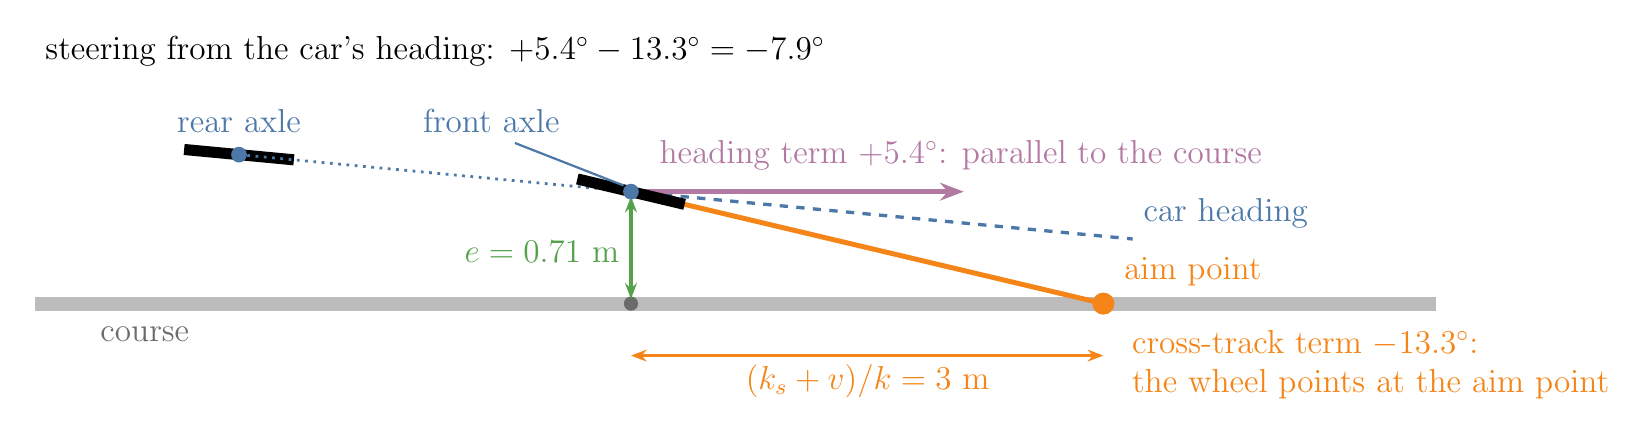
\begin{tikzpicture}[scale=2.0, every node/.append style={font=\large}]
  % course
  \draw[cgrey!45, line width=5pt] (-0.3,0) -- (8.6,0);
  \node[cgrey, anchor=north] at (0.4,-0.08) {course};
  % rear wheel and wheelbase
  \begin{scope}[shift={(0.998,0.946)}, rotate=-5.39]
    \draw[black, line width=4pt] (-0.35,0) -- (0.35,0);
    \draw[cblue, dotted, line width=1pt] (0,0) -- (2.5,0);
  \end{scope}
  \fill[cblue] (0.998,0.946) circle (0.05);
  \node[cblue, anchor=south] at (0.998,1.02) {rear axle};
  % car heading through the front axle
  \draw[cblue, dashed, line width=1.2pt] (3.487,0.711) -- ++(-5.39:3.2);
  \node[cblue, anchor=south west] at ($(3.487,0.711)+(-5.39:3.2)$) {car heading};
  % nearest point and lateral error at the front axle
  \fill[cgrey] (3.487,0) circle (0.045);
  \draw[cgreen, line width=1.4pt, {Stealth[length=2mm]}-{Stealth[length=2mm]}] (3.487,0.03) -- (3.487,0.68);
  \node[cgreen, anchor=east, fill=white, inner sep=1pt] at (3.44,0.33) {$e = 0.71$ m};
  % heading term: parallel to the course
  \draw[-{Stealth[length=3mm]}, cpurple, line width=1.8pt] (3.487,0.711) -- (5.6,0.711);
  \node[cpurple, anchor=south west] at (3.6,0.78) {heading term $+5.4^\circ$: parallel to the course};
  % cross-track term: towards the aim point 3 m ahead of the nearest point
  \draw[corange, line width=1.8pt] (3.487,0.711) -- (6.487,0);
  \fill[corange] (6.487,0) circle (0.07);
  \node[corange, anchor=south west] at (6.55,0.04) {aim point};
  \node[corange, anchor=north west, align=left] at (6.6,-0.1) {cross-track term $-13.3^\circ$:\\the wheel points at the aim point};
  % distance along the course to the aim point
  \draw[corange, line width=1pt, {Stealth[length=2mm]}-{Stealth[length=2mm]}] (3.487,-0.33) -- (6.487,-0.33);
  \node[corange, anchor=north, fill=white, inner sep=1pt] at (4.99,-0.36) {$(k_s + v)/k = 3$ m};
  % front wheel along the commanded direction
  \draw[black, line width=4pt] ($(3.487,0.711)+(-13.34:-0.35)$) -- ($(3.487,0.711)+(-13.34:0.35)$);
  \fill[cblue] (3.487,0.711) circle (0.05);
  \node[cblue, anchor=south] at (2.6,1.02) {front axle};
  \draw[cblue, line width=0.8pt] (2.75,1.02) -- (3.44,0.75);
  % result
  \node[black, anchor=west] at (-0.3,1.6) {steering from the car's heading: $+5.4^\circ - 13.3^\circ = -7.9^\circ$};
\end{tikzpicture}
\end{document}
